\section{LDA}

Wie gefordert wurden die normale Variante und die Fisher-Variante der LDA implementiert.

\paragraph{Normale LDA}
Bei der normalen LDA berechnet sich der Transformationsvektor zu $\vect{w} \propto (\overline{m_2} - \overline{m_1})$ mit den Klassenmittelwerten $\overline{m_k} = \frac{1}{N_k} \sum_{\overline{x_n} \in C_k} \overline{x_n}$. Die dimensionsreduzierten Werte ergeben sich dann zu $\hat{x} = \vect{w}^T x$.

\paragraph{Fisher-LDA}
Bei der Fisher-LDA berechnet sich der Transformationsvektor zu $\vect{w} \propto S_W^{-1} (\overline{m_2} - \overline{m_1})$ mit den Klassenmittelwerten $\overline{m_k} = \frac{1}{N_k} \sum_{\overline{x_n} \in C_k} \overline{x_n}$ und der \emph{within-Covarianzmatrix} $S_W = \sum_{k = 1}^K \sum_{n = 1}^N (x_n - \overline{m_k}) (x_n - \overline{m_k})^T$, wobei $k$ die Klassennummer, $K$ die Gesamtanzahl an Klassen, $n$ der Elementindex, $N$ die Gesamtanzahl an Elementen und $N_k$ die Anzahl an Elementen in der Klasse $C_k$ angibt. Die dimensionsreduzierten Werte ergeben sich dann zu $\hat{x} = \vect{w}^T x$.


Abbildungen \ref{fig:4_2_lda_data} und \ref{fig:4_2_fisher_data} zeigen die Punktewolken der beiden Klassen $C_1$ und $C_2$ für LDA und Fisher-LDA. Man erkennt, dass die normale LDA nur die Mittelwerte der Klassen berücksichtigt, und alle Datenpunkte auf den Vektor $\vect{w}$ projiziert, der die Mittelpunkte verbindet. Im Gegensatz dazu berücksichtigt die Fisher-Variante auch die Streuung innerhalb der Klassen, wodurch die Klassen besser separierbar sind.

\begin{figure}[hp!]
\begin{center}
 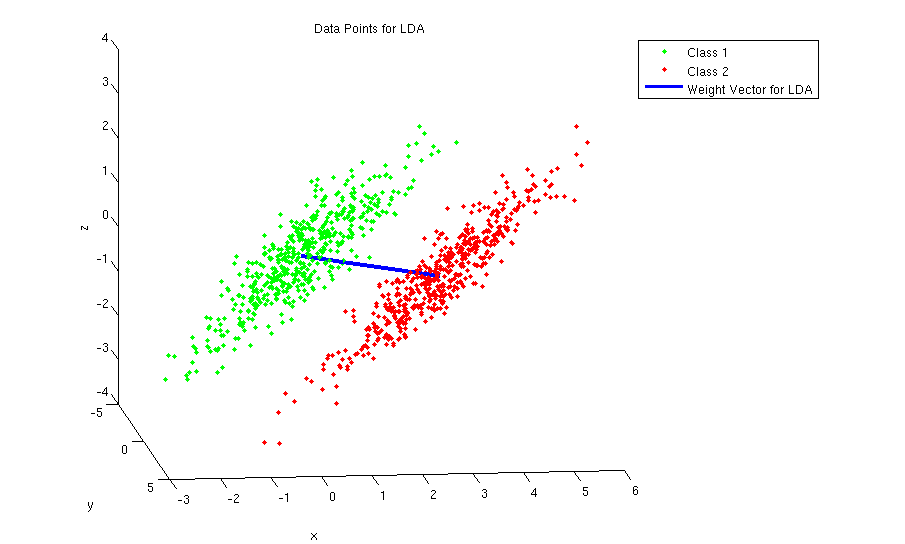
\includegraphics[width=\textwidth]{./figures/4_2_lda_data}
 \caption{Datenpunkte der beiden Klassen und Transformationsvektor für LDA}
\label{fig:4_2_lda_data}
\end{center}
\end{figure}

\begin{figure}[hp!]
\begin{center}
 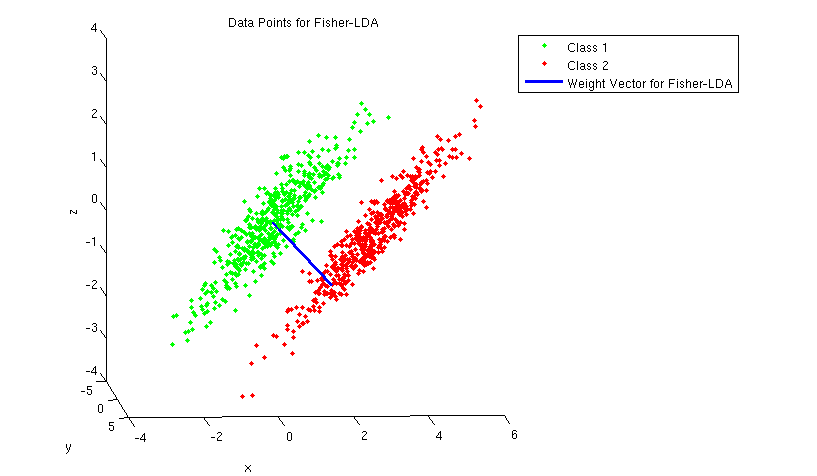
\includegraphics[width=\textwidth]{./figures/4_2_fisher_data}
 \caption{Datenpunkte der beiden Klassen und Transformationsvektor für Fisher-LDA}
\label{fig:4_2_fisher_data}
\end{center}
\end{figure}


Abbildungen \ref{fig:4_2_lda_1d} und \ref{fig:4_2_lda_hist} zeigen die projizierten Daten und das Histogramm der Daten nach der LDA. Man erkennt im Histogramm, dass sich die projizierten Klassen überlappen und dadurch nur schlecht separierbar sind. Berechnet man die Erkennrate einer Klassifizierung nach der normalen LDA ($\frac{\textrm{ Anzahl richtig klassifizierter Elemente }}{\textrm{ Gesamtanzahl der Elemente }}$, Threshold ist schwarz gepunktet im Histogramm eingezeichnet, ergibt sich aus dem Minimum des Gesamthistogramms zwischen den beiden Peaks), ergibt sich folgendes Ergebnis: \texttt{LDA: Threshold is 5.5188, Performance on Class 1 is 0.948, Performance on Class 2 is 0.954, Overall Performance is 0.951}. Die Erkennrate ist also in diesem Beispiel $95.4\%$.

\begin{figure}[hp!]
\begin{center}
 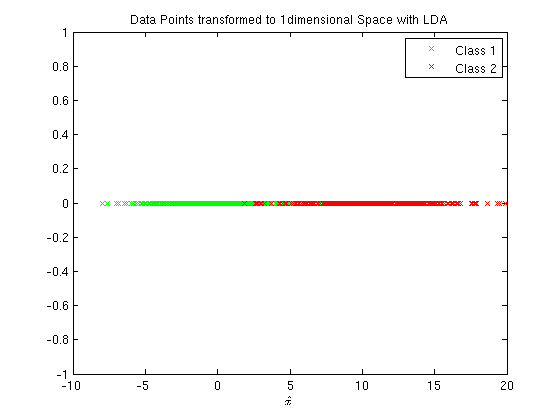
\includegraphics[width=0.75\textwidth]{./figures/4_2_lda_1d}
 \caption{Projizierte Datenpunkte für LDA}
\label{fig:4_2_lda_1d}
\end{center}
\end{figure}

\begin{figure}[hp!]
\begin{center}
 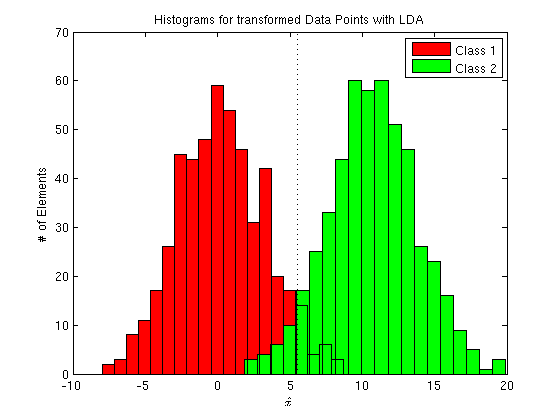
\includegraphics[width=0.75\textwidth]{./figures/4_2_lda_hist}
 \caption{Histogramm für LDA mit eingezeichnetem Threshold}
\label{fig:4_2_lda_hist}
\end{center}
\end{figure}


Abbildungen \ref{fig:4_2_fisher_1d} und \ref{fig:4_2_fisher_hist} zeigen die projizierten Daten und das Histogramm der Daten nach der Fisher-LDA. Man erkennt im Histogramm, dass sich die projizierten Klassen nicht überlappen und dadurch gut separierbar sind. Berechnet man die Erkennrate einer Klassifizierung nach der Fisher-LDA ($\frac{\textrm{ Anzahl richtig klassifizierter Elemente }}{\textrm{ Gesamtanzahl der Elemente }}$, Threshold ist schwarz gepunktet im Histogramm eingezeichnet, ergibt sich aus dem Minimum des Gesamthistogramms zwischen den beiden Peaks), ergibt sich folgendes Ergebnis: \texttt{Fisher-LDA: Threshold is 0.027209, Performance on Class 1 is 1, Performance on Class 2 is 1, Overall Performance is 1}. Die Erkennrate ist also in diesem Beispiel $100\%$.

\begin{figure}[hp!]
\begin{center}
 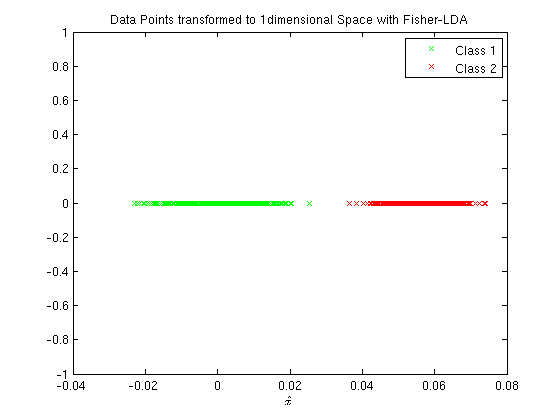
\includegraphics[width=0.75\textwidth]{./figures/4_2_fisher_1d}
 \caption{Projizierte Datenpunkte für Fisher-LDA}
\label{fig:4_2_fisher_1d}
\end{center}
\end{figure}

\begin{figure}[hp!]
\begin{center}
 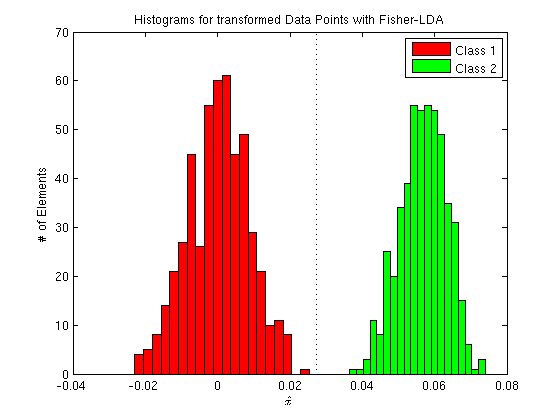
\includegraphics[width=0.75\textwidth]{./figures/4_2_fisher_hist}
 \caption{Histogramm für Fisher-LDA mit eingezeichnetem Threshold}
\label{fig:4_2_fisher_hist}
\end{center}
\end{figure}


\paragraph{Unterschied zur PCA}

Die PCA findet wie der Name sagt die Hauptkomponenten in einer Menge von Datenpunkten. Zur Dimensionsreduktion kann man die Datenpunkte nach der PCA auf die Hauptkomponentenrichtung projizieren und erhält dadurch eine maximale Varianz in den projizierten Daten. Jegliche Klassenzuordnungen werden bei der PCA ignoriert. Die PCA ist also hauptsächlich ein Verfahren zur Dimensionsreduktion.

Die LDA jedoch nimmt Rücksicht auf die Klassenzugehörigkeit der einzelnen Datenpunkte. Bei der LDA werden Vektoren berechnet, die nach einer Projektion eine möglichst gute Separierbarkeit und dadurch eine möglichst gute Klassifikation der Daten ermöglichen. Die LDA ist also ein Klassifikationsverfahren.

